\documentclass[tikz, border=5pt]{standalone}
\usepackage{tikz}
\usetikzlibrary{calc,positioning,intersections,shadows.blur,decorations.pathmorphing,patterns,shapes.callouts}

\definecolor{moonGray}{RGB}{180,180,180}
\definecolor{craterGray}{RGB}{120,120,120}
\definecolor{spaceBlue}{RGB}{10,10,40}
\definecolor{beige}{RGB}{245,245,220}

\begin{document}
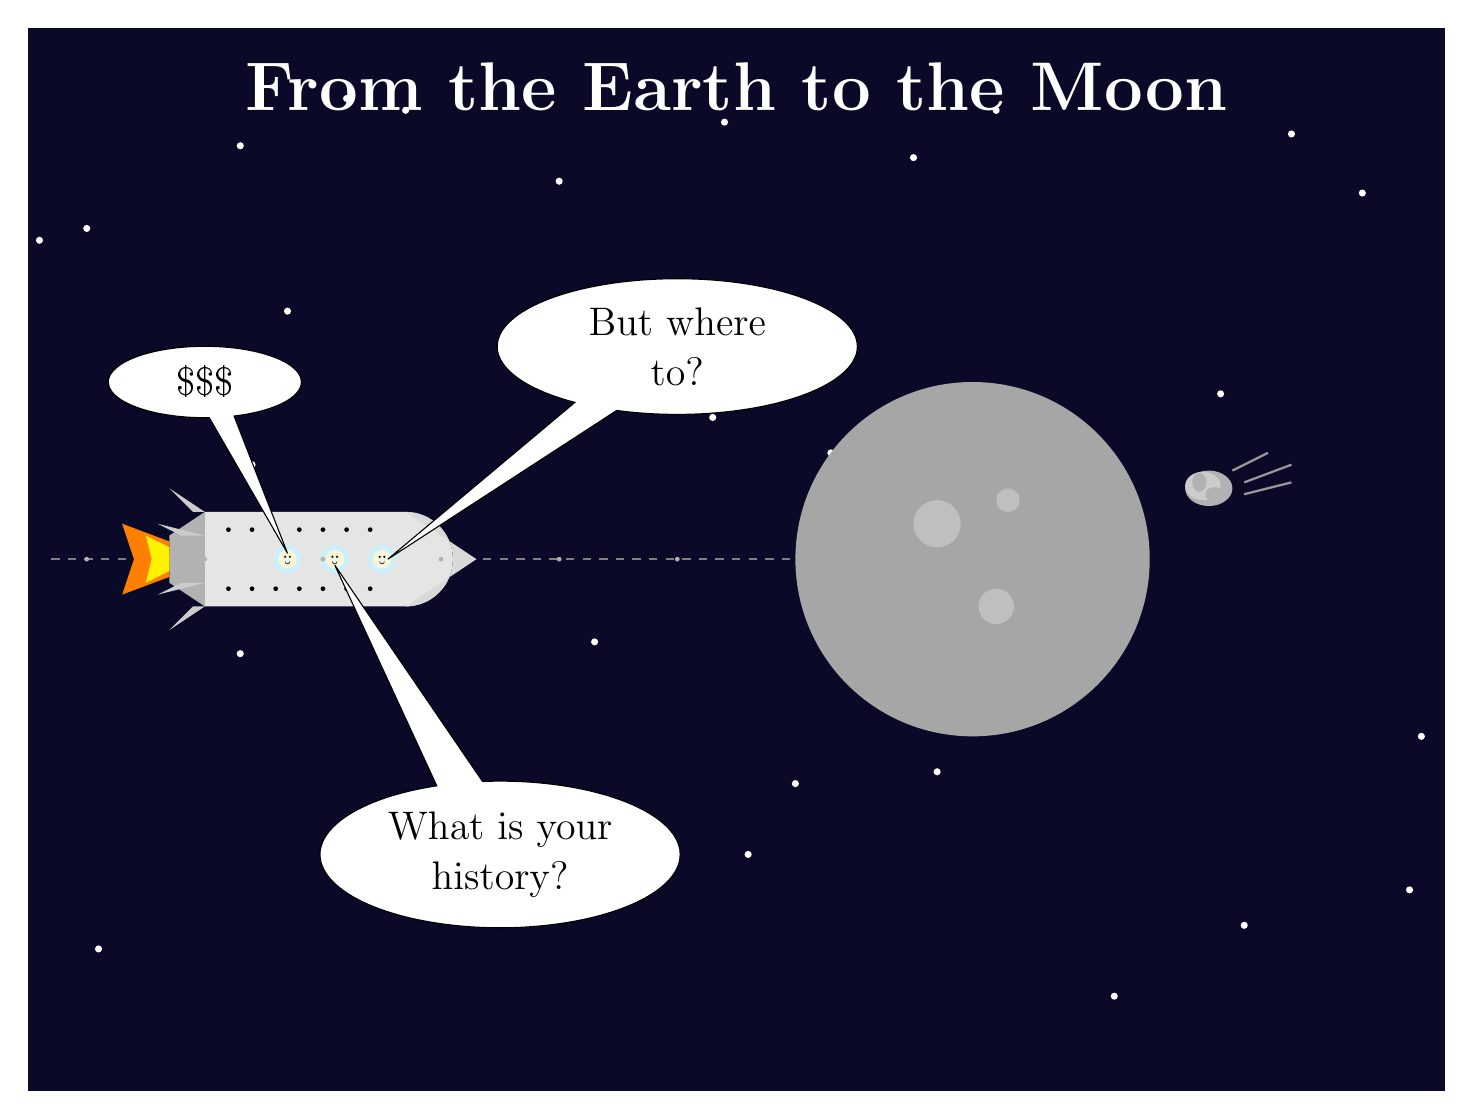
\begin{tikzpicture}[scale=1.5]

% Background (space)
\fill[spaceBlue] (-4,-4.5) rectangle (8,4.5);

% Title
\node[white, font=\Huge\bfseries, align=center] at (2,4) {From the Earth to the Moon};

% Straight trajectory showing path to the moon
\draw[gray, dashed, thick] (-3.8,0) -- (2.5,0);

% Add some stars (adjusted coordinates for the new background size)
\foreach \x/\y in {-3.5/2.8, -2.2/3.5, -1.8/2.1, 0.5/3.2, 1.8/1.8, 2.1/-2.5, 6.3/-3.1, 7.7/-2.8, 0.5/1.8, 2.8/0.9, 4.2/3.8, 6.1/1.4, 7.3/3.1, -3.9/2.7, -2.1/0.8, -1.3/3.9, 1.8/1.2, 3.5/3.4, 3.7/-1.8, 5.2/-3.7, 7.8/-1.5, -3.4/-3.3, 2.5/-1.9, 0.8/-0.7, 4.8/-0.3, -2.2/-0.8, 3.1/-0.4, 1.9/3.7, 6.7/3.6, -0.8/3.8} {
  \fill[white] (\x,\y) circle (0.03);
}

% Moon
\fill[gray!70] (4,0) circle (1.5cm);
\fill[gray!50] (3.7,0.3) circle (0.2cm);
\fill[gray!50] (4.2,-0.4) circle (0.15cm);
\fill[gray!50] (4.3,0.5) circle (0.1cm);

% Spacecraft body (bullet/projectile shape) - fixed hull
\fill[gray!20] (-2.5,0.4) -- (-0.8,0.4) arc (90:-90:0.4) -- (-2.5,-0.4) -- cycle;
\fill[gray!60] (-2.5,0.4) -- (-2.8,0.2) -- (-2.8,-0.2) -- (-2.5,-0.4) -- cycle;

% Nose cone (pointed front) - fixed shape
\fill[gray!30] (-0.8,0.4) arc (90:-90:0.4) -- (-0.2,0) -- cycle;

% Viewing windows with small heads including happy mouths
\fill[cyan!20] (-1.8,0) circle (0.12cm);
\fill[beige] (-1.8,0) circle (0.08cm);
\fill[black] (-1.82,0.02) circle (0.01cm);
\fill[black] (-1.78,0.02) circle (0.01cm);
\draw[black, very thin] (-1.78,-0.02) arc (180:0:-0.02cm);

\fill[cyan!20] (-1.4,0) circle (0.12cm);
\fill[beige] (-1.4,0) circle (0.08cm);
\fill[black] (-1.42,0.02) circle (0.01cm);
\fill[black] (-1.38,0.02) circle (0.01cm);
\draw[black, very thin] (-1.38,-0.02) arc (180:0:-0.02cm);

\fill[cyan!20] (-1,0) circle (0.12cm);
\fill[beige] (-1,0) circle (0.08cm);
\fill[black] (-1.02,0.02) circle (0.01cm);
\fill[black] (-0.98,0.02) circle (0.01cm);
\draw[black, very thin] (-0.98,-0.02) arc (180:0:-0.02cm);

% Rivets/bolts along the hull
\foreach \x in {-2.3, -2.1, -1.9, -1.7, -1.5, -1.3, -1.1} {
    \fill[black] (\x,0.25) circle (0.02cm);
    \fill[black] (\x,-0.25) circle (0.02cm);
}

% Fins/stabilizers at the back
\fill[gray!40] (-2.5,0.4) -- (-2.8,0.6) -- (-2.6,0.4) -- cycle;
\fill[gray!40] (-2.5,-0.4) -- (-2.8,-0.6) -- (-2.6,-0.4) -- cycle;
\fill[gray!40] (-2.5,0.2) -- (-2.9,0.3) -- (-2.7,0.2) -- cycle;
\fill[gray!40] (-2.5,-0.2) -- (-2.9,-0.3) -- (-2.7,-0.2) -- cycle;

% Thruster flames from the back
\fill[orange] (-2.8,0.15) -- (-3.2,0.3) -- (-3.1,0) -- (-3.2,-0.3) -- (-2.8,-0.15) -- cycle;
\fill[yellow] (-2.8,0.1) -- (-3.0,0.2) -- (-2.95,0) -- (-3.0,-0.2) -- (-2.8,-0.1) -- cycle;

% Speech bubbles pointing to each person
% First bubble pointing to leftmost person
\node[ellipse callout, draw, fill=white, callout absolute pointer={(-1.8,0.05)}, 
      text width=1.5cm, align=center, font=\Large] at (-2.5,1.5) {\$\$\$};

% Second bubble pointing to middle person
\node[ellipse callout, draw, fill=white, callout absolute pointer={(-1.4,-0.05)}, 
      text width=3cm, align=center, font=\Large] at (0,-2.5) {What is your history?};

% Third bubble pointing to rightmost person
\node[ellipse callout, draw, fill=white, callout absolute pointer={(-0.95,0)}, 
      text width=3cm, align=center, font=\Large] at (1.5,1.8) {But where to?};

% Add some trajectory markers to show direction
\foreach \x in {-3.5, -2.5, -1.5, -0.5, 0.5, 1.5} {
    \fill[gray!60] (\x, 0) circle (0.02cm);
}

% Large meteorite about to impact on the back side of the moon (irregular shape, moved further from impact)
\fill[gray!60] (6.0,0.6) ellipse (0.2cm and 0.15cm);
\fill[gray!40] (5.95,0.62) ellipse (0.15cm and 0.12cm);

% Irregular asteroid shape details
\fill[gray!60] (6.05,0.55) ellipse (0.08cm and 0.06cm);
\fill[gray!60] (5.92,0.65) ellipse (0.06cm and 0.08cm);

% Movement lines indicating trajectory toward moon center
\draw[gray!80, thick] (6.5,0.9) -- (6.2,0.75);
\draw[gray!80, thick] (6.7,0.8) -- (6.3,0.65);
\draw[gray!80, thick] (6.7,0.65) -- (6.3,0.55);

\end{tikzpicture}
\end{document}